\section{Introduction and scope}

\subsection{Project goal}

RatMan is a maze-chase game for Windows. The player steers a rat through a maze, collects cheese, and tries to clear the board before the cats take all three lives. The project also gives board creators a way to design levels inside the application. A custom layout can change where the player encounters a cat, which routes are available, and how quickly a round becomes difficult.

The goal was to build a complete C\# desktop application spanning gameplay, interface design, and local persistence. The project also demonstrates the course topics through concrete implementation and verification examples \cite{exam,project}.

\subsection{Delivered scope}

A player can start with the bundled Classic map or select a saved map from the library. During a round, the interface shows the current score, lives, cheese progress, and cat status. Collecting all cheese wins the round, and losing the last life ends it. The player can replay the same layout or return to the menu. A qualifying score can be saved with an optional name and appears on the leaderboard for that layout. Leaving an unfinished round returns directly to the menu.

The board builder supports editing dimensions, walls, border tunnels, spawns, and cheese. Saved boards become available from the map library and can be reopened for further editing. Movement has two configurable keys per direction, so players can keep the arrow keys, use WASD, or choose another set. Together, these features cover the path from creating a board to playing and comparing scores across repeated attempts. Figure~\ref{fig:gameplay} illustrates the two parts of the gameplay screen that make the round readable.

\reportfigure{fig:gameplay}{A round in progress on the Packman board. The sidebar shows score, lives, and cat status.}{%
  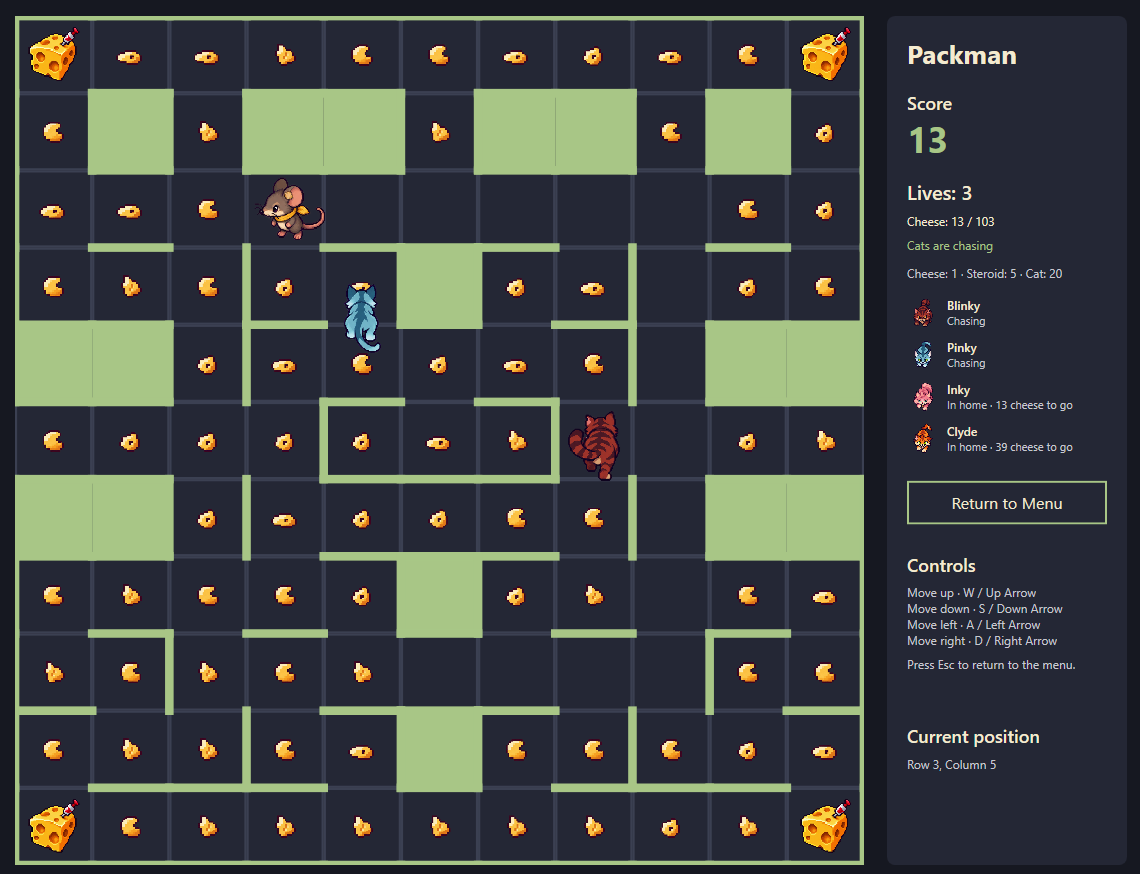
\includegraphics[width=\linewidth,height=77mm,keepaspectratio]{img/fig1.png}}

\clearpage
\section{Architecture and WPF}

\subsection{Solution and assembly boundaries}

The solution separates the responsibility for deciding what happens in a round from the responsibility for displaying it. \code{RatMan.Game} builds into \code{RatMan.Game.dll}, a .NET 10 library containing the maze topology, actor motion, and gameplay rules. Its public types use logical coordinates, directions, and elapsed time. The engine can therefore run the same scenario in a unit test or in the desktop application with the same rules. For example, a tunnel crossing can be verified independently of the sprite that represents it.

\code{RatMan.App} builds into the Windows-targeted \code{RatMan.dll}. It references the engine and owns the WPF views, view models, animation, and local repositories. The test project references both components. That lets the suite exercise pure engine behavior and also check the view models and selected WPF visuals. Figure~\ref{fig:projects} shows the current dependency directions.

A managed assembly packages compiled code and type metadata. It can also carry embedded resources. The WPF project embeds \code{Classic.maze} under a manifest resource name. When the maze library is initialized, \code{FileMazeRepository} uses the assembly that contains its own type to open the named resource stream and seed the map file. The bundled map consequently travels with the application assembly, and the saved copy can then be edited like other maps.

\reportfigure{fig:projects}{Solution dependencies. Arrows point to referenced projects.}{%
  \begin{tikzpicture}
  \node[ratman box] (tests) at (0,1.45)
    {\textbf{\code{RatMan.Tests}}\\MSTest suite};
  \node[ratman box] (app) at (-3.65,-1.05)
    {\textbf{\code{RatMan.App}}\\\mbox{Windows WPF application}};
  \node[ratman box] (engine) at (3.65,-1.05)
    {\textbf{\code{RatMan.Game}}\\WPF-independent library};

  \draw[ratman arrow] (tests.south west) -- (app.north);
  \draw[ratman arrow] (tests.south east) -- (engine.north);
  \draw[ratman arrow] (app.east) -- (engine.west);
\end{tikzpicture}
}

\clearpage
\subsection{Navigation, commands, and binding}

The interface follows Model--View--ViewModel (MVVM) \cite{mvvm}. The model defines the game rules, the view describes the visual layout, and the view model exposes the state and actions needed by XAML. The main window binds a \code{ContentControl} to \code{ActiveScreen}. Application-level data templates match the active view model's type to its corresponding view. A menu action can therefore switch screens by changing one property.

WPF buttons use the \code{ICommand} contract. RatMan implements it through \code{RelayCommand}. Its \code{Action<object?>} delegate executes the command. An optional \code{Predicate<object?>} delegate determines when it is available. The view model supplies the behavior, often as a lambda, and the view binds to the resulting command. For example, Replay becomes available when a round has finished and the application is free to start another. A change in status prompts WPF to recheck command availability. Inheritance also shares common behavior. \code{GameViewModel} derives from \code{ScreenViewModel}, which supplies a title and inherits property notification from \code{ObservableObject}.

The score illustrates the return path to the interface. After the session advances, the game view model copies the engine's score into its bindable property. A changed value raises \code{PropertyChanged}, which lets the score text update. WPF builds views from XAML and handwritten C\# using partial classes. The handwritten constructor calls the generated \code{InitializeComponent} method, and \code{GameView} handles keyboard focus and the rendering clock as part of its view lifecycle.

\subsection{Board rendering and sprites}

The game view places tiles, walls, food, and actors in layered Canvas visuals. The view models convert logical positions and movement progress into pixel coordinates. WPF bindings then position each element, and a view box scales the board to the available space. A separate sidebar presents the round's state alongside the board. The sprite presenter chooses a clip from the actor's facing direction and state. A clip defines rectangular crops and frame durations. The animation code advances playback with elapsed time and reuses cached image crops. Separate position and frame calculations let a sprite animate while its game position follows the same rules as any actor. Figure~\ref{fig:gameplay} shows the resulting layers, and Figure~\ref{fig:gameplay-flow} shows when presentation updates are applied.

\clearpage
\section{Game engine and maze design}

\subsection{Domain model and invariants}

\code{MazeDefinition} describes the starting layout, including dimensions, walls, spawn positions, openings, and food overrides. Its validation checks that the two spawns occupy different cells, that walls separate adjacent cells inside the board, and that food overrides are consistent. \code{GameSession} constructs the runtime state from a validated maze. It initializes its topology, actors, and starting food, then keeps the state that changes during the round.

Encapsulation makes the session responsible for score and lives. Both properties have private setters. The session awards points when an eligible item is collected and decrements lives when a dangerous contact occurs. Callers observe those properties and request actions through methods. This keeps the same rules in effect for keyboard input and test drivers.

\code{GridPosition} is a \code{readonly record struct}. Two values with the same row and column compare equal, so a position can identify a food item in a typed dictionary regardless of where the value came from. Its generic parameters, \code{GridPosition} and \code{FoodKind}, specify the key and value types at compile time. The read-only public view of that dictionary allows presentation code to inspect the food that remains. Figure~\ref{fig:domain} summarizes the model relationships.

\reportfigure{fig:domain}{Starting maze data and mutable round state. Dashed arrows identify uses of the grid position value.}{%
  \begin{tikzpicture}[
  domain node/.style={ratman box, minimum width=3.05cm, minimum height=1.20cm},
  position link/.style={ratman arrow, dashed}
]
  \node[domain node] (maze) at (-5.0,1.8)
    {\textbf{\code{MazeDefinition}}\\Starting layout and spawns};
  \node[domain node] (session) at (0,1.8)
    {\textbf{\code{GameSession}}\\Rules, score, lives};
  \node[domain node] (topology) at (5.0,1.8)
    {\textbf{\code{BoardTopology}}\\Legal steps and reachability};

  \node[domain node] (player) at (-5.0,-0.55)
    {\textbf{\code{Player}}\\RatMan's movement};
  \node[domain node] (cats) at (0,-0.55)
    {\textbf{\code{Cat}}\\State and movement};
  \node[domain node] (food) at (5.0,-0.55)
    {\textbf{Remaining food}\\Tile-to-food dictionary};

  \node[domain node] (position) at (0,-3.0)
    {\textbf{\code{GridPosition}}\\Row and column value};

  \draw[ratman arrow] (maze.east) -- node[ratman label, above] {initializes} (session.west);
  \draw[ratman arrow] (session.east) -- node[ratman label, above] {uses} (topology.west);
  \draw[ratman arrow] (session.south) -- node[ratman label, right, pos=.72] {owns 0 or 4} (cats.north);
  \draw[ratman arrow] (0,0.64) -- node[ratman label, above] {owns 1} (-5.0,0.64) -- (player.north);
  \draw[ratman arrow] (0,0.64) -- node[ratman label, above] {stores} (5.0,0.64) -- (food.north);

  \draw[position link] (player.south) -- (-5.0,-2.1) -- node[ratman label, above] {actor position} (-1.1,-2.1) -- ([xshift=-1.1cm]position.north);
  \draw[position link] (cats.south) -- node[ratman label, right] {actor position} (position.north);
  \draw[position link] (food.south) -- (5.0,-2.1) -- node[ratman label, above] {tile key} (1.1,-2.1) -- ([xshift=1.1cm]position.north);
  \draw[position link] (maze.west) -- (-7.35,1.8) -- (-7.35,-3.0)
    -- node[ratman label, above] {spawn positions} (position.west);
\end{tikzpicture}
}

\clearpage
\subsection{Input and fixed-step simulation}

Keyboard input and game time enter through separate paths. The view checks the pressed key against the configured movement bindings. The view model converts a recognized key to a direction request, and the engine stores the latest request as a pending turn. Separately, WPF's rendering event supplies elapsed time through \code{RenderingClock}. The clock caps a long frame at 100 milliseconds, and the session advances as many 10-millisecond simulation steps as the accumulated time allows, retaining the remainder for the next update. Figure~\ref{fig:gameplay-flow} shows how the paths meet.

Consider RatMan moving right along a corridor. Pressing Up while travelling towards a tile with a wall above it queues Up. When the rat reaches that tile, the turn is still unavailable, so it continues right. If the following tile opens upward, the engine can start the pending turn there. When the rat completes a move onto a tile with ordinary cheese, the engine removes that cheese and awards one point. Removing the entry also prevents later movement across that tile from awarding the same point again. The view model then updates the displayed position, remaining food, and score.

The fixed step also makes the order of contact and arrival testable. For example, a cat crossing the rat's path partway along an edge is handled before food at the destination is collected. Tests can drive the session with explicit elapsed times and check the resulting state without waiting for screen frames.

\reportfigure{fig:gameplay-flow}{Keyboard input and render updates meet in the game session.}{%
  \begin{tikzpicture}[
  participant/.style={ratman box, minimum width=2.85cm, minimum height=0.73cm},
  lifeline/.style={draw=muted, densely dashed, thin},
  phase/.style={anchor=west, fill=white, inner xsep=4pt, font=\sffamily\small\bfseries, text=accent}
]
  \node[participant] (view) at (0,0) {\textbf{\code{GameView}}};
  \node[participant] (clock) at (3.35,0) {\textbf{\code{RenderingClock}}};
  \node[participant] (vm) at (6.7,0) {\textbf{\code{GameViewModel}}};
  \node[participant] (session) at (10.3,0) {\textbf{\code{GameSession}}};

  \foreach \actor in {view,clock,vm,session}
    \draw[lifeline] (\actor.south) -- ++(0,-7.30);

  \draw[rulecolor] (-1.38,-0.78) -- (12.02,-0.78);
  \node[phase] at (-1.28,-0.78) {Keyboard event};
  \draw[ratman arrow] (0,-1.47) -- node[ratman label, above] {Resolve binding and execute \code{MoveCommand}} (6.7,-1.47);
  \draw[ratman arrow] (6.7,-2.18) -- node[ratman label, above] {\code{RequestDirection(direction)}} (10.3,-2.18);
  \draw[ratman arrow] (10.3,-2.43) -- ++(0.65,0) -- ++(0,-0.48)
    -- node[ratman label, left, pos=1] {Store latest pending turn} (10.3,-2.91);

  \draw[rulecolor] (-1.38,-3.36) -- (12.02,-3.36);
  \node[phase] at (-1.28,-3.36) {WPF render callback};
  \draw[ratman arrow] (3.35,-4.05) -- node[ratman label, above] {\code{Advance(capped elapsed)}} (6.7,-4.05);
  \draw[ratman arrow] (6.7,-4.77) -- node[ratman label, above] {\code{Advance(elapsed)}} (10.3,-4.77);

  \node[ratman box, font=\sffamily\footnotesize, text width=4.75cm, minimum height=0pt] at (9.35,-5.62)
    {Accumulate time and run one step per 10 ms. On arrival, collect cheese and update the score.};
  \draw[ratman arrow, dashed] (10.3,-6.94) -- node[ratman label, above] {Updated game state} (6.7,-6.94);
  \draw[ratman arrow] (6.7,-7.63) -- node[ratman label, above] {Synchronize presentation and notify bindings} (0,-7.63);
\end{tikzpicture}
}

\clearpage
\subsection{Board builder, tunnels, and reachability}

The maze is a grid whose walls are edges between adjacent cells. Movement within the board is legal when the edge between the current and destination cell is open. An opening at the boundary is represented by its row or column, so both opposing borders open together. A step through one side re-enters on the other. The same \code{BoardTopology.TryStep} method applies both rules.

The board builder recomputes the cells reachable from the player spawn when the layout changes. A breadth-first search uses a \code{Queue<GridPosition>} to process pending cells and a \code{HashSet<GridPosition>} to record each cell as it is discovered. The visited set prevents repeated work even when a path returns through the same tunnel. The editor shades inaccessible cells and hides their cheese, while preserving food overrides so that they can take effect if the cells become reachable again.

Figure~\ref{fig:reachability} uses an editor test with a three-column, two-row board. A wall immediately after the first column leaves four cells inaccessible from the player spawn. Opening the opposing borders in the upper row makes those cells reachable even though the divider stays in place. Cats also use the topology. Their navigator builds a breadth-first distance map from a reachable target and uses it to choose among legal exits. The \code{Opposite()} extension method helps exclude reversal during ordinary navigation, with exceptions for dead ends and the return-home route. The same model therefore determines the editor preview, the player's available moves, and the cats' routes on a custom board.

\reportfigure{fig:reachability}{Board Builder before and after opening the upper-row tunnel. The divider stays in place while the four shaded cells become reachable.}{%
  \begingroup
\newcommand{\reachabilityboard}[2]{%
  \resizebox{\linewidth}{!}{%
    \begin{tikzpicture}
      \path[use as bounding box] (-0.28,0) rectangle (7.90,6.03);
      % The captures are 1046 x 913; retain the 762 x 518 board region.
      \begin{scope}
        \clip (0,0) rectangle (7.62,5.18);
        \node[anchor=south west,inner sep=0] at (-0.12,-1.82)
          {\includegraphics[width=10.46cm]{#1}};
      \end{scope}
      #2
    \end{tikzpicture}}%
}
\begin{minipage}[t]{0.477\linewidth}
  \centering
  \reachabilityboard{img/fig5-closed.jpg}{}
  \par\smallskip
  {\sffamily\small\textbf{A. Tunnel closed}\\2 of 6 cells reachable}
\end{minipage}\hfill
\begin{minipage}[t]{0.477\linewidth}
  \centering
  \reachabilityboard{img/fig5-open.jpg}{%
    \draw[draw=accent,semithick,{Latex[length=2.0mm]}-{Latex[length=2.0mm]},rounded corners=4pt]
      (0.03,3.88) -- (-0.21,3.88) -- (-0.21,5.58) --
      node[ratman label,above] {Paired tunnel} (7.83,5.58) -- (7.83,3.88) -- (7.59,3.88);
  }
  \par\smallskip
  {\sffamily\small\textbf{B. Tunnel open}\\6 of 6 cells reachable}
\end{minipage}
\endgroup
}

\clearpage
\subsection{Cat behavior and round outcomes}

The cat logic separates target selection from the search for a route. In chase mode, \code{GameSession} calls \code{ICatTargetStrategy.Target} through the same interface for every cat. Blinky targets RatMan's current cell. Pinky uses the rat's facing direction to aim ahead. The strategy implementations give each cat a different pursuit behavior while sharing the navigator. The navigator resolves an unreachable target to a reachable cell and uses a fixed priority to break ties between exits.

Blinky releases immediately. The remaining cats release after enough cheese has been collected. Their thresholds are 10, 25, and 50 percent of the starting food count, rounded up to whole pieces. Steroid cheese activates a ten-second power period that sends active cats into scatter mode. Contact with a scattering cat awards points and sends it home, harmless while returning. A cat that reaches home during power waits in recovery until power expires. Figure~\ref{fig:cat-states} groups these transitions around release, contact, and the power timer.

Contact with a chasing cat costs a life. If one remains, the engine pauses briefly and resets the actors to their starting positions while retaining the score, collected cheese, and release progress. The final life lost produces Game Over. Collecting the last cheese produces victory. The terminal state stops game progression and lets the view model raise the round-completion event. Replay restores food and resets the score and lives for the same layout. Keeping the round outcome separate from the cats' states allows a cat's return-home behavior and the player's life count to evolve independently.

\reportfigure{fig:cat-states}{Cat states during a round. Resetting the actors returns cats to Waiting and rechecks their release thresholds.}{%
  \begin{tikzpicture}[
  state/.style={ratman box, minimum width=2.55cm, minimum height=0.77cm, font=\sffamily\small\bfseries}
]
  \node[state] (waiting) at (0,2.2) {Waiting};
  \node[state] (chase) at (-3.83,0.35) {Chase};
  \node[state] (scatter) at (3.83,0.35) {Scatter};
  \node[state] (returning) at (3.83,-2.05) {Returning home};
  \node[state] (recovering) at (0,-3.78) {Recovering};

  \draw[ratman arrow] (waiting.south west) -- (chase.north);
  \draw[ratman arrow] (waiting.south east) -- (scatter.north);
  \node[ratman label, align=center] at (-3.65,1.77) {Threshold met\\(power off)};
  \node[ratman label, align=center] at (3.65,1.77) {Threshold met\\(power active)};

  \draw[ratman arrow] ([yshift=2mm]chase.east) -- node[ratman label, above] {Power starts} ([yshift=2mm]scatter.west);
  \draw[ratman arrow] ([yshift=-2mm]scatter.west) -- node[ratman label, below] {Power expires} ([yshift=-2mm]chase.east);
  \draw[ratman arrow] (scatter.south) -- node[ratman label, right] {Contact with RatMan} (returning.north);

  \draw[ratman arrow] (returning.west) -- node[ratman label, above] {Home [power off]} (-3.83,-2.05) -- (chase.south);
  \draw[ratman arrow] (returning.south west) -- (recovering.north east);
  \node[ratman label] at (3.55,-3.13) {Home [power active]};
  \draw[ratman arrow] (recovering.west) -- node[ratman label, above] {Power expires} (-5.7,-3.78)
    -- (-5.7,0.35) -- (chase.west);
\end{tikzpicture}
}

\clearpage
\section{Persistence and concurrency}

\subsection{Local files and failure handling}

RatMan stores its data under the current Windows user's local application-data folder. The map library holds versioned \code{.maze} files containing JSON. The other files store movement bindings and leaderboard entries. Files store the information needed to restore settings, boards, and completed scores. In-progress actor positions and the current round score belong to the session.

The maze loader accepts version~1 and version~2. Version~2 adds food overrides. The loader gives older files default food, and a later save writes the version~2 shape. It translates JSON parsing failures into an \code{InvalidDataException}. The catalog catches file errors per map and records the affected entry as invalid, so valid maps are still available for play.

When saving a leaderboard, the repository writes a complete JSON snapshot to a temporary file and then replaces the destination. Until replacement succeeds, the saved destination is kept intact. The inner \code{finally} block attempts to clean up the temporary file, and the outer one releases the synchronization gate even after an exception. High-score reads validate the payload before submission can rewrite it. The game can report an unreadable leaderboard and offer a retry. If saving a new score fails, the dialog keeps the name available so the player can retry or skip.

\subsection{Per-layout leaderboards and LINQ}

Once a round reaches a terminal state, \code{GameViewModel} raises \code{RoundCompleted} with the final score, a completion identifier, the time, and the outcome. A lambda in \code{MainViewModel} subscribes and starts the qualification check. If the score places in the top ten, the app offers name entry. The leaderboard substitutes Anonymous for a blank name. The repository checks qualification again when submitting, because the ranking can change between opening the dialog and saving.

The leaderboard key is a hash of canonical gameplay data, including dimensions, spawns, walls, tunnels, and effective starting food. Wall and food entries are sorted before hashing so their order in a file has no effect on the key. Renaming a maze preserves the key. An edit that changes the playable layout produces a separate leaderboard. This keeps comparisons tied to the board on which the score was earned. Returning a board to a previous layout also restores its association with earlier scores.

The ranking uses LINQ over in-memory entries. \code{OrderByDescending} sorts by score and retains the input order for ties. The new entry is appended, so previously saved scores keep priority at the same value. \code{Take} limits the result to ten and \code{ToArray()} enumerates the query into a snapshot. For database-backed storage, Entity Framework Core could map leaderboard records to entities, let a provider translate supported LINQ operations, and persist tracked changes through \code{SaveChanges} \cite{ef-query,ef-save}. Versioned JSON suits the local workload because the app reads and rewrites small collections and can set up its storage on first use.

\clearpage
\subsection{Threading and async I/O}

The WPF UI thread runs the game view's rendering callback, drives the session, and applies the resulting presentation changes. The engine processes each step serially to preserve the defined ordering of movement, contact, and scoring. A task awaiting file I/O can yield to the UI while the operation is incomplete. That is asynchronous progress, distinct from CPU parallelism, which would schedule game calculations to run simultaneously. Shared game state and the small board sizes make serial updates a practical choice.

The high-score repository serializes submissions targeting the same file within the process by awaiting a per-path \code{SemaphoreSlim}. It also opens a lock file with exclusive sharing to guard against another app process writing during the read, rank, and replace sequence. This protects the whole update, since two writers could otherwise read the same old ranking and each write a snapshot missing the other's entry.

The application runs in the default AppDomain of its .NET process. Earlier .NET Framework applications could create additional AppDomains in the same process. Modern .NET gives the process one AppDomain, and RatMan loads its statically referenced components in the normal assembly load context \cite{domains}. The process boundary also explains why the in-memory semaphore needs a separate mechanism for coordinating file access across instances.

\clearpage
\section{Verification and development process}

\subsection{Automated verification}

The Windows MSTest suite at application revision \code{c0c7c88} completed with 208 passes, zero failures, and zero skips. It covers game rules, storage, view models, and selected WPF rendering behavior. Table~\ref{tab:verification} shows representative cases and the behavior each one checks. The tunnel test checks the destination at the opposite edge. The collision test places steroid cheese beyond a contact occurring during movement and checks that losing a life prevents collection. The storage test starts submissions from ten repository instances targeting one temporary file and reloads the ranking to check that all ten scores survived in descending order.

The rendering test also validates an observable result of arrival. The score text stays at zero halfway through a move and becomes five when the player reaches a steroid cheese tile. This checks the connection between the fixed-step model and the WPF binding.

MSTest uses attributes such as \code{[TestClass]} and \code{[TestMethod]} as discovery metadata. The rendering test creates a single-threaded apartment (STA) thread for its WPF objects. The test waits for that thread to finish and propagates a failure. Within the rendering test, reflection locates the private \code{renderingClock} field by name at runtime and reads its value. The test checks that repeated loading replaces the clock, that unloading stops it, and that the field is cleared. This illustrates late binding in a concrete test, with a maintenance trade-off because a field rename also changes the lookup.

\begin{table}[h!]
  \centering
  \caption{Representative results from the Windows test run.}
  \label{tab:verification}
  \small
  \renewcommand{\arraystretch}{1.18}
  \begin{tabularx}{\linewidth}{@{}>{\raggedright\arraybackslash}p{0.20\linewidth}
    >{\raggedright\arraybackslash}X
    >{\raggedright\arraybackslash}p{0.22\linewidth}
    >{\raggedright\arraybackslash}p{0.11\linewidth}@{}}
    \toprule
    Scenario & Expected behavior & Method & Result \\
    \midrule
    Border tunnel & The actor arrives at the opposite edge through an open border. & Topology test & Pass \\
    Contact before arrival & An earlier collision prevents collection of cheese on the unreached cell. & Gameplay test & Pass \\
    Concurrent submissions & Ten repository instances preserve all ten qualifying entries in score order. & Repository test & Pass \\
    View unloading & The clock stops and the view clears its reference. & WPF rendering test & Pass \\
    \bottomrule
  \end{tabularx}
\end{table}

\clearpage
\subsection{Verification scope and limitations}

Fixed-step engine tests can reproduce contact near a tile boundary, a power timer expiring, or an actor entering a tunnel. Repository tests create temporary files and exercise compatibility and recovery separately from the app's normal data. The WPF rendering case checks selected controls and lifecycle behavior in a controlled environment. Those layers provide evidence about rules, persistence, and binding. Overall difficulty, the feel of keyboard controls, and the clarity of the status panel across longer rounds are questions for playtesting.

The application is a Windows desktop program because the interface uses WPF. Leaderboards compare attempts stored in one local Windows profile. In a course project this keeps deployment and storage simple. A shared leaderboard would have to define how distinct users and simultaneous submissions are handled across machines.

\subsection{Human-supervised AI use}

AI assistance was used to speed up development. Its value was in shortening the time from a defined task to a candidate solution that could be evaluated. It can help explore an implementation approach, produce an initial draft, or suggest where to investigate a problem. The developer supplies the goal, relevant project context, and expected behavior. Those decisions give the developer a basis for judging whether the result fits RatMan.

Human supervision applies to both the proposed design and the resulting changes. The developer reviews suggestions in the context of the existing code, checks that the relevant requirements and invariants are preserved, and revises or discards outputs that conflict with them. Builds and targeted tests supply evidence for behavior that can be checked automatically. Changes involving timing or persistence need particular attention to the order of events and the handling of errors. A passing test is a check of a specific expectation, and the developer still decides which expectations need to be exercised.

The developer remains responsible for accepting changes and for explaining the resulting implementation at the examination. The development benefit is qualitative. AI reduces some of the effort involved in exploring and drafting a candidate, while the time for review and verification remains part of the work. Project decisions and the evidence for them remain attributable to the developer.

\clearpage
\section{Conclusion}

RatMan delivers a complete desktop maze chase with editable boards, configurable movement, and persistent leaderboards tied to the layout played. The automated suite supports the main design claims with tests of engine rules, file handling, and selected WPF behavior. The project brings the course topics together through a single application, from the use of value types and events to the handling of overlapping file operations.

The main architectural lesson is that an explicit boundary around the game rules makes behavior easier to reason about and verify. A test can reproduce a precise sequence of movement and contact using elapsed time, while the interface can render the same behavior with its own layout and animation. That boundary also gives the board builder and cat navigation a shared definition of which moves are legal, keeping the editor and game consistent.
